\documentclass{article}
\usepackage[utf8]{inputenc}

\title{ngspice01}
\author{antoine.remy99 }
\date{March 12 2020}
\usepackage{graphicx}
\usepackage{auto-pst-pdf}
\begin{document}

\maketitle

\section{GSchem}

I started this project by creating a gschem document to create my circuit I used one voltage generator and 2 resistor :
\\
-Resistor 1 as a value of  27\begin{math}\Omega\end{math}
\\
-Resistor 2 as a value of 127.\begin{math}\Omega\end{math}
\\
-Voltage generator as a value of 54V .\newline

And I linked all the component to obtain this :
\begin{center}
    \includegraphics[scale = 0.25,angle=270]{picture/01.ps}
\end{center}

I finally transformed the .sch into a .net by using gnetlist.\\

the file net file was :\\
\begin{verbatim}
* Spice netlister for gnetlist
V1 1 0 54
R2 0 2 127
R1 1 2 27
.END
\end{verbatim}

\section{NGspice}

After exporting the .sch into a .net using gnetlist.\\
I used ngspice to calculate the different voltage of all the resistors by using command :
    -tran  5 1
    -plot "1"
    -plot "2"
    as show below:


\begin{center}
    \includegraphics[scale = 0.25]{picture/011.ps}\\
    \textbf{Resistor 1}\\
    \includegraphics[scale = 0.25]{picture/012.ps}\\
    \textbf{Resistor 2}
\end{center}

\section{Conclusion}

This work allow me to learn how to create electrical circuit in GSchem and to evaluate them using NGspice.
\end{document}
